% !TEX encoding = UTF-8
% !TEX TS-program = pdflatex
% !TEX root = ../tesi.tex

%**************************************************************
\chapter{Parsing Details\label{app:par}}
%**************************************************************

	In this appendix, we give more details about the parser and how we understood how it works. 
	The original parser we worked on is available on Valve's GitHub page in the repository named csgo-demoinfogo\footnote{\href{https://github.com/ValveSoftware/csgo-demoinfo}{https://github.com/ValveSoftware/csgo-demoinfo}}.
	Since there is no documentation, we had to experiment a lot to understand it. 
	The first thing we noticed is that the parser relies on protobuf messages\footnote{\href{https://github.com/protocolbuffers/protobuf}{https://github.com/protocolbuffers/protobuf}}. 
	After downloading protobuf, we were able to compile the parser and run it. 
	We discovered that the parser logged everything on the console, so we redirected the output to a \emph{txt} file to analyze it. 
	During the analysis of the parser, we noticed that information was saved in some data structures that were called tables by the programmers. 
	The parsing divided entities (which are the players' controlled characters) and actions (performed by the players).
	In Figure \ref{fig:ent}, there is an example of a parsed entity.
	
	\begin{figure}[!h] 
		\centering 
		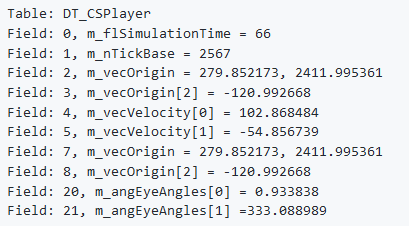
\includegraphics[scale=.8]{parser/original_entity.png}
		\caption{\label{fig:ent}Example of parsed entity.}
	\end{figure}
	
	The first thing we wanted to understand was the logic used, and what the parser saved in the tables. 
	Looking at Figure \ref{fig:ent}, we find some interesting variables dumped. 
	
	\begin{itemize}
	
		\item \texbtbf{Player's position}:\\			
			The variable \texttt{m\_vecOrigin}, contained in 2 couple of fields, contains the player's position relative to the $(0,0,0)$ coordinate of the map. 
			The first field of the couple contains an array of length 2 that memorizes the $X$ and $Y$ coordinate respectively, the other field of the couple memorized the $Z$ coordinate. \\
	
		\item \textbf{Player's speed}:\\
			The variable \texttt{m\_vecVelocity} is an array of length 3 that memorizes the speed of the player along the three axes ($X$, $Y$, and $Z$). 
			It is worth mentioning that at index 0 there is the $X$ axis' speed, at index 1 the $Z$ axis' speed, and at index 2 the $Y$ axis' speed.
	
		\item \textbf{Camera position}:\\
			The variable \texttt{m\_angEyeAngles}, contained in fields 20 and 21, contains two angles (used probably in a 3D polar coordinate system), which represent the position of the mouse and the camera movement. 
			The fact that these variables are angles, thus scaled in a $[0, 360)$ interval, is very useful because results in two variables with equal domain for every user. 
			
	\end{itemize}

	Focusing more on the action, in Figure \ref{fig:act2} there is an example of parsed action.
	
	\begin{figure}[!h] 
		\centering 
		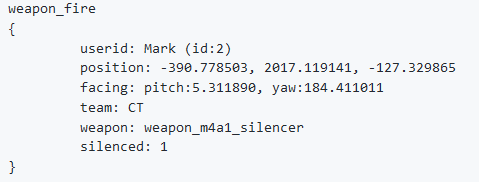
\includegraphics[width=.9\columnwidth]{parser/original_action.png}
		\caption{\label{fig:act2}Example of parsed action.}
	\end{figure}
	
	Focusing on the actions, we thought that every action had a unique id predefined by the game. 
	Parsing different matches, though, we found that the actions' id changed from game to game. 
	At the same time, we noticed that every event has its descriptors, and, in particular, the name used in said descriptors is always the same. 
	We can see, in Figure \ref{fig:act2}, how the action parsed has some properties. 
	The most important is the \texttt{userid}, which represents the id of the user that performed the action. 
	This one, along with the team, are the only common fields through all the actions. 
	Concerning the crouch state, we found that it was treated as an entity property, not as an action. 
	The game keeps track of the offset along the $Y$ axis that represents the crouch state. 
	So we decided to dump the offset and keep track of it as an entity property.\\
	We needed to find a way to keep track of the entity and the actions performed by the player we wanted to analyze. 
	The problem we faced was that entities and actions used two different ids, called \texttt{entityId} and \texttt{id} respectively. 
	So we had to understand how the game gives the id to the player and the entities. 
	We found that it uses the \texttt{steamId}, a unique id in the \gls{Steam} platform. 
	So we decided to create a \emph{.h} file to share the player's data between multiple files. 
	Using this technique, we could share both the \texttt{entityId} and the \texttt{id}, along with all the entity's information, like the position, the speed, the $Y$ offset, and the camera position. 
	This decision helped us to also dump the speed of the player every time the parser output some text since we discovered that the speed was dumped only if there were any changes. 
	Once we created and assigned the values to this file, we modified the parser with some simple if statements. 
	Before every dumping we needed, we checked if the dumped entity was the one we were interested in. 
	In case the parser was dumping an action if the action was one of the ones we wanted  (using the event's name) to keep and if it was performed by the player we were following. 
	With this simple modification, we were able to modify the parser's output and only dump the informations regarding the player we were interested in.
